\section{\ac{bus} images segmentation using optimization}\label{sec:methodApp}
In this section, the problem of delineating structures in \ac{bus} images is defined as an optimization problem that can be solved applying the framework presented in Sect.\,\ref{sec:method}.
The segmentation here proposed aims at tying a label $l\in\mathcal{L}$ (\emph{i.e.} $\{\text{lesion}, \overline{\text{lesion}}\}$ or $\{ \text{chest wall}, \text{lungs}, \dots, \text{lesion} \}$) to each element of $\mathcal{S}$ by simultaneously optimizing the data and pairwise terms as illustrated in Fig.\,\ref{fig:methodTerms}.
Choices made regarding these different elements:
the representation $\mathcal{S}$, the data term $D(\cdot)$, the pairwise term $V(.)$, and the optimizer choice are summarized in Table~{\color{red}??} and justified thereafter (see Fig.\,\ref{fig:method} for reference).

$\mathcal{S}$ is considered the result from an over-segmentation of the image using Quick-shift super-pixel~\cite{achanta2012slic}. 
The structures of the breast and their rendering when using a hand-held 2D \ac{us} probe are sketched in Fig.\,\ref{fig:features}a. Figure~\ref{fig:features}b illustrates the lexicon proposed by the \ac{acr}~\cite{biradsus} and used by clinicians to perform their diagnosis. Thus, our aim is to generate a set of computer vision features which is able to encode the characteristic described in the lexicon. The selected features are the following:

\begin{figure}[t]
  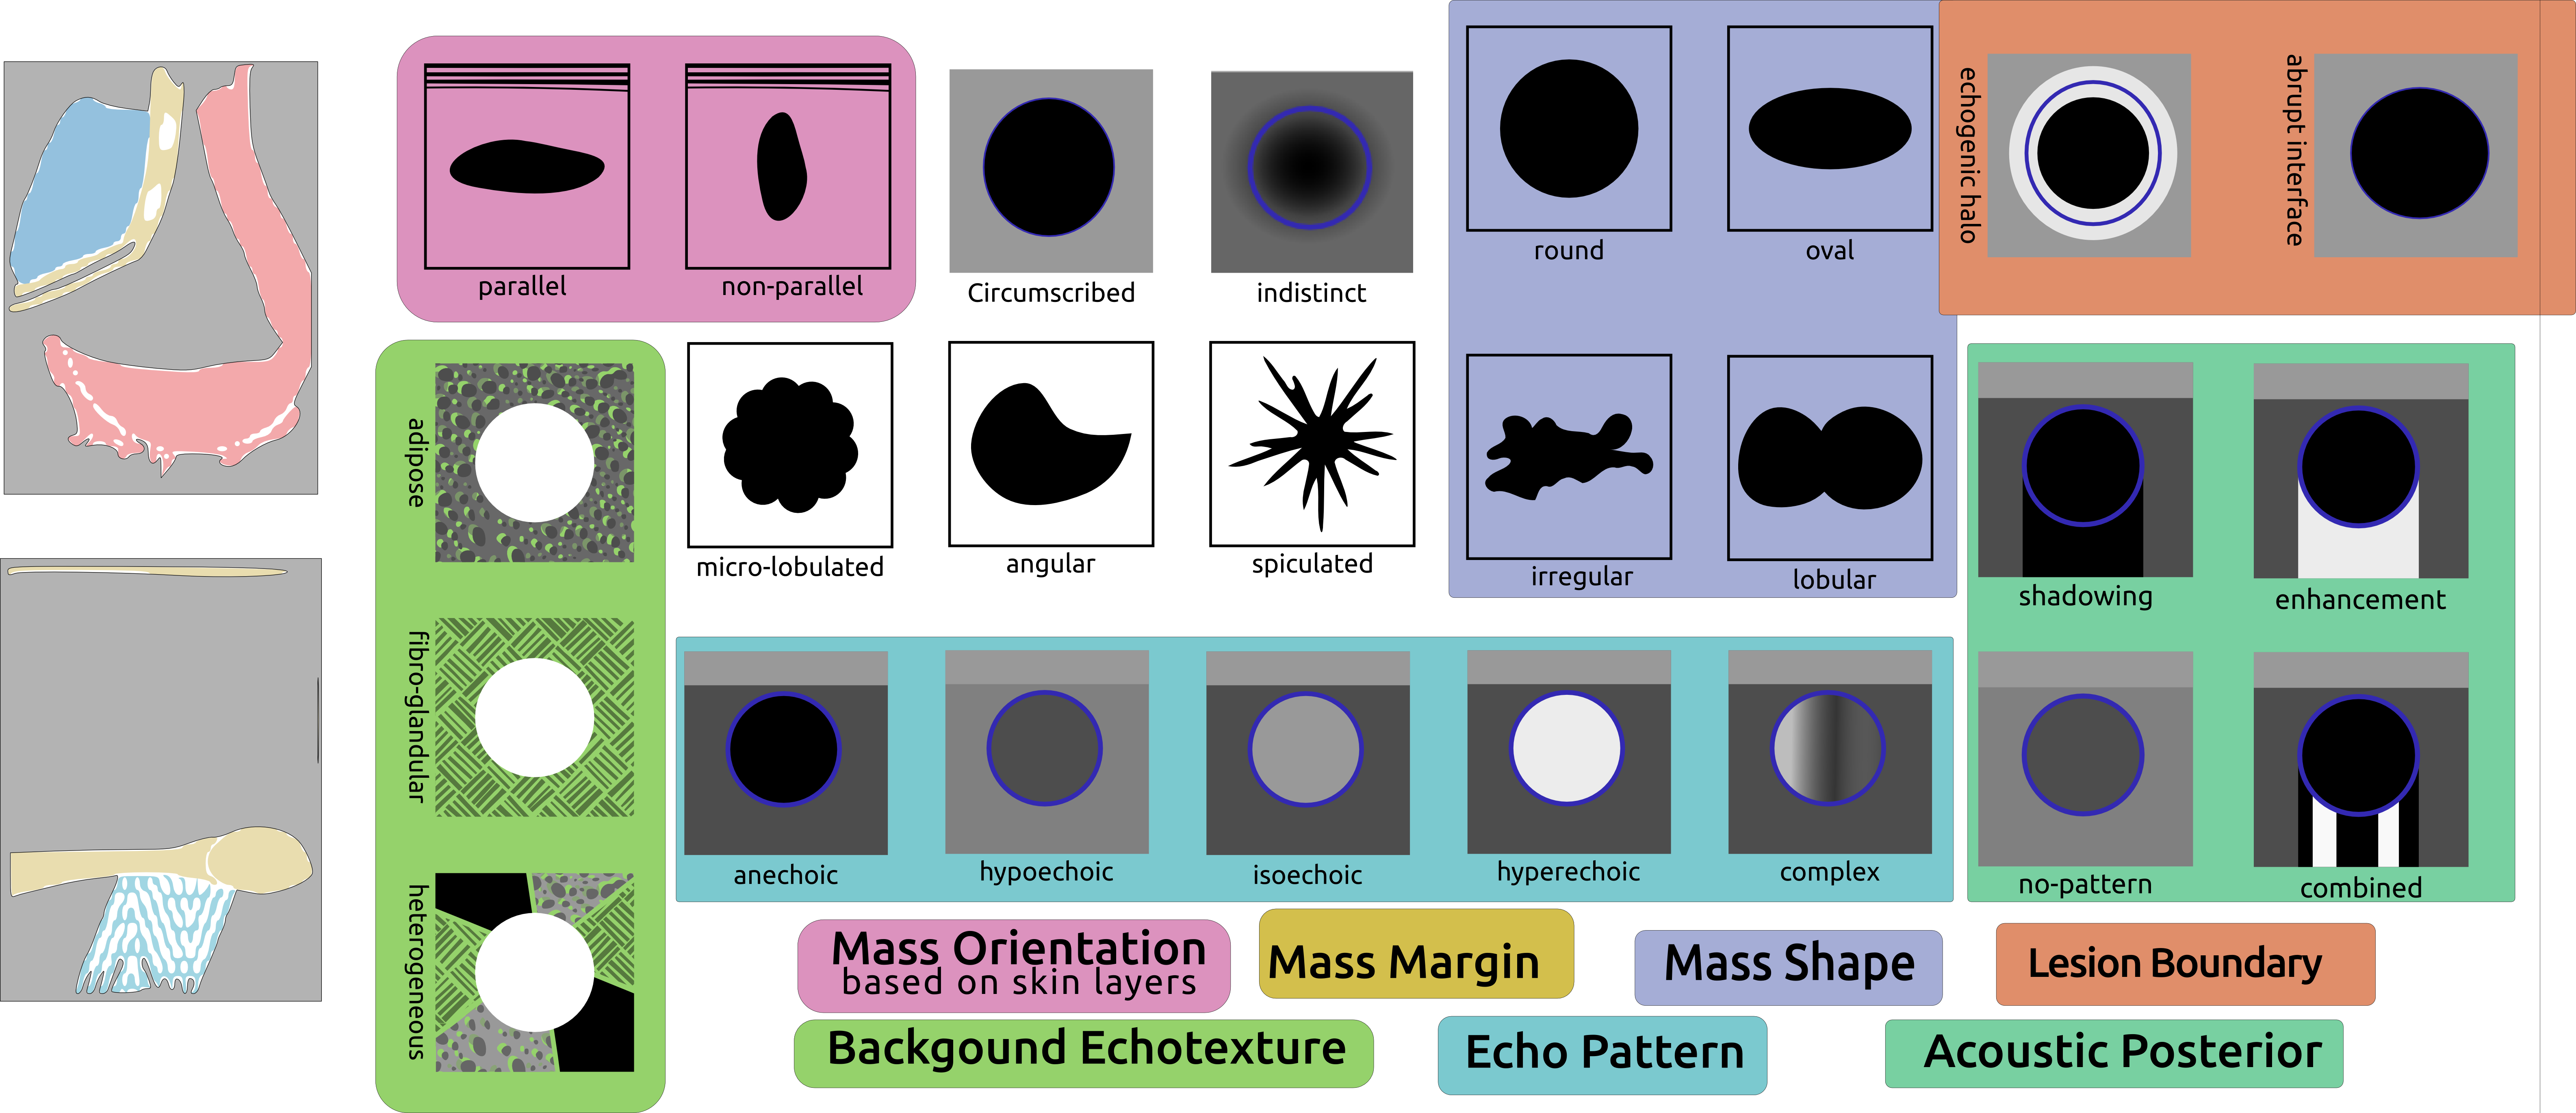
\includegraphics[width=0.9\textwidth]{lexiconReworked}
    \caption {{\footnotesize Visual reference: (a) breast structures, (b) US BI-RADS lexicon, (c) encoded visual cues.}} 
    \label{fig:features}
\end{figure}




\begin{description}
  \item[Appearance] 
    Based on the multi-labelled \ac{gt}, a \ac{mad} histogram model for every tissue label is built. The Appearance feature is computed as the $\chi^2$ distance between a histogram of $s$ and the models generated.
  \item[Atlas] 
    Based on the multi-labelled \ac{gt} an atlas is build to encode the labels likelihood based on the location of $s$.
  \item[Brightness] 
    Intensity descriptors are computed based on statistics of $s$ (\emph{i.e:} mean, median, mode) and  are compared with some intensity markers of the set $\mathcal{S}$ such as the minimum intensity value, the maximum, its mean, etc.
  \item[\ac{sift}-\ac{bof}]
    $s$ is described as an histogram of visual words based on \ac{sift}~\cite{massich2014sift}. The dictionary is built with $36$ words.
\end{description}

The relationships between the lexicon and the descriptors previously described is depicted in Table~{\color{red}??}. More precisely, we highlight the corresponding elements of the lexicon which is encoded by each feature. A choice regarding the encoding of the data term $D(\cdot)$ has to be made by using a \ac{ml} classifier. An \ac{svm} classifier with an \ac{rbf} kernel is selected to determine the data model during the training stage. The pairwise term is our framework was defined as in Eq.\,\eqref{eq:smoothing}. The optimization method used as solver to minimize our cost function $U(\cdot)$ is \ac{gc}. \ac{gc} when applicable allows to rapidly find a strong local minima guaranteeing that no other minimum with lower energies can be found~\cite{delong2012fast}. \ac{gc} is applicable if, and only if, the pairwise term favours coherent labelling configurations and penalizes labelling configurations where neighbours labels differs; such is our case, given by Eq.\,\eqref{eq:smoothing}.

%%% Local Variables: 
%%% mode: latex
%%% TeX-master: "../../master"
%%% End: 
